\section{Referencial Teórico}
	\subsection{Materiais}
	\subsubsection{FPGA}
	\begin{frame}{FPGA}
		\centering \color{blue} {\Huge \textbf{FPGA} \\[0.5cm]}% {\huge FPGA}
	\end{frame}
	\begin{frame}{FPGA}
		\begin{itemize}
  			\setlength\itemsep{1em}
		%It consists of an array of logic blocks and routing channels. Two I/O pads fit into the height of one row or the width of one column, as shown below. All the routing channels have the same width (number of wires). 
			\item Tocci (2003) cita que os dispositivos lógicos programáveis são as ``\textit{maravilhas de flexibilidade de projeto}''.
			\item FPGA (\textit{Field Programmable Gate Array}, ou seja, Arranjo de Portas Programável em Campo) consiste num \textbf{arranjo de blocos lógicos} e \textbf{canais de roteamento}.
			\item Significa que é capaz de alterar seus caminhos de dados/fluxos \textbf{habilitando/desabilitando módulos} \cite{moreira2008plataforma}.
		\end{itemize}
	\end{frame}
	\begin{frame}{FPGA - Roteamento de Blocos}
		\begin{figure}[p]
			\centering
			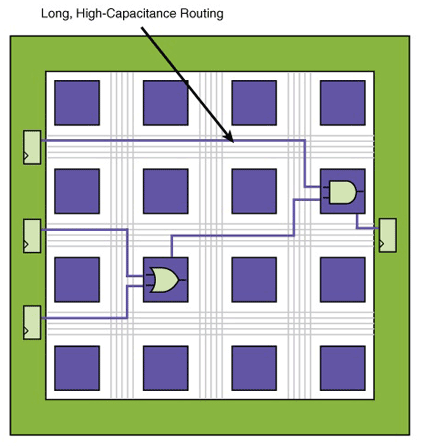
\includegraphics[width=0.55\textwidth]{img/fpga/exemploInicial.png}
			\caption{Exemplo de roteamento interno no FPGA.}
			\label{fig:fpgaHardware}
		\end{figure}
	\end{frame}
	%\begin{frame}{FPGA - Roteamento de Blocos}
	%	\begin{figure}[p]
	%		\centering
	%		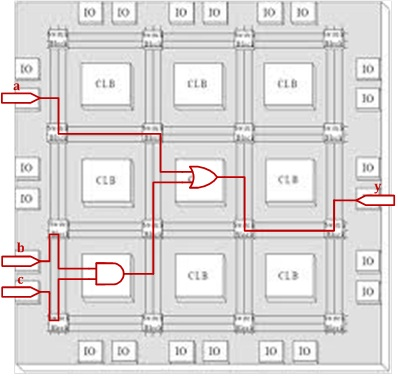
\includegraphics[width=0.6\textwidth]{img/fpga/exemplo.jpg}
	%		\caption{Outro exemplo de roteamento interno no FPGA.}
	%		\label{fig:fpgaHardware}
	%	\end{figure}
	%\end{frame}
	\begin{frame}%{FPGA - Roteamento de Blocos}
		\begin{figure}[p]
			\centering
			\includegraphics[width=0.64\textwidth]{img/fpga/exemploFinal.png}
			\caption{Exemplo de roteamento interno bastante complexo no FPGA..}
			\label{fig:fpgaHardware}
		\end{figure}
	\end{frame}
	\begin{frame}{FPGA - Placa}
		\begin{figure}[p]
			\centering
			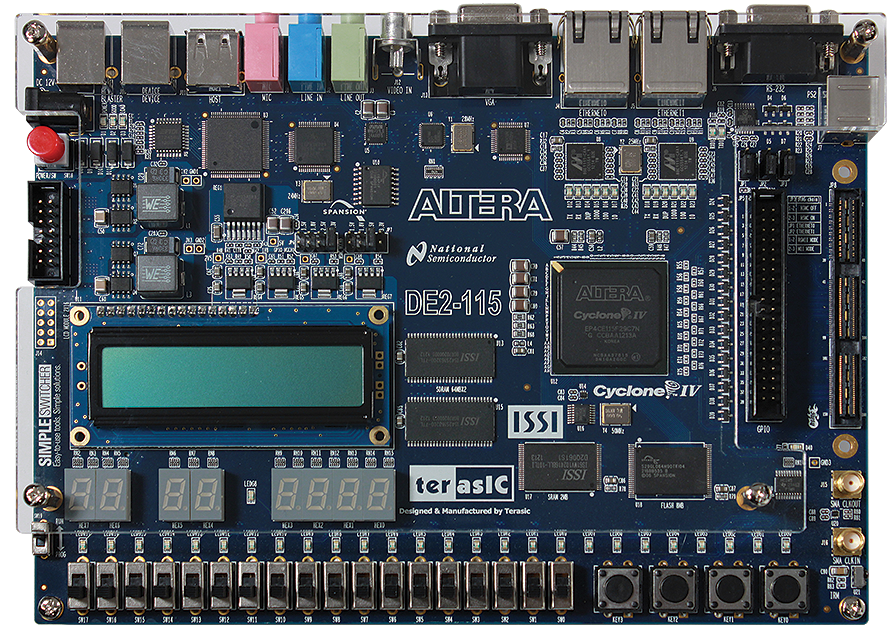
\includegraphics[width=0.8\textwidth]{img/fpgaHardware.png}
			\caption{FPGA de Desenvolvimento Altera DE2-115.}
			\label{fig:fpgaHardware}
		\end{figure}
	\end{frame}
	\begin{frame}
		\begin{figure}[p]
			\centering
			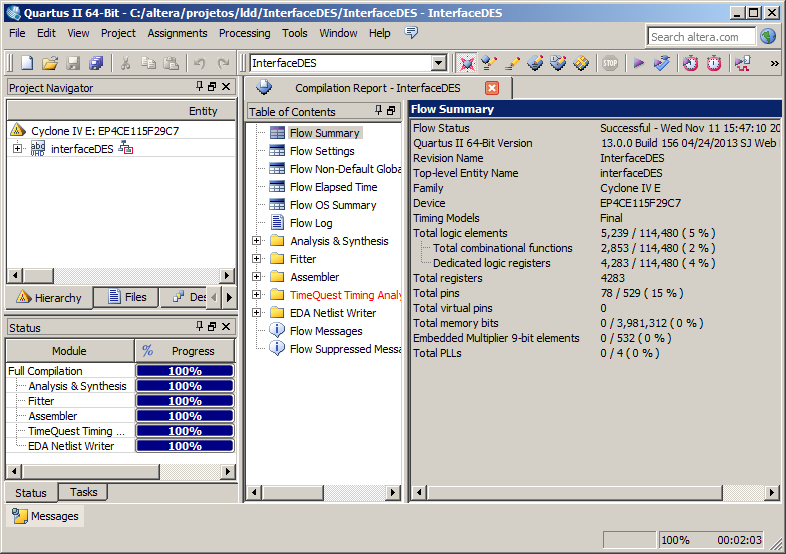
\includegraphics[width=0.97\textwidth]{img/fpga/altera.png}
			\caption{Altera Quartus II.}
			\label{fig:fpgaHardware}
		\end{figure}
	\end{frame}
	\begin{frame}{FPGA}
		\begin{itemize}
			\item Características importantes da placa utilizada:
			\begin{itemize}
  				\setlength\itemsep{1em}
				\item \textbf{Altera DE2-115} utilizada para ensino e desenvolvimento.
				\item Quantidade de elementos lógicos: 114.480;
				\item IDE\footnote{Integrated Development Environment ou Ambiente de Desenvolvimento Integrado.} Quartus II;
				\item Utilizou-se a linguagem de descrição de \textit{hardware} VHDL;
				\begin{itemize}
					\item \textit{VHSIC Hardware Description Language}, ou seja, uma linguagem de descrição de hardware VHSIC\footnote{\textit{Very High Speed Integrated Circuits.}}.
				\end{itemize}
				\item \textit{Clock} de $50Mhz$;
				\item \textbf{Várias interfaces} para acomodar as mais diversas aplicações.
			\end{itemize} 
			\bigskip
			\item São muito utilizados para \textbf{desenvolver protótipos} e \textbf{realização de testes} antes da fabricação em massa \cite{skliarova2003introduccao}.
		\end{itemize}
	\end{frame}

%	\begin{frame}{Saleae Logic16}
%	\end{frame}

	\subsubsection{Arduino}
	\begin{frame}{Arduino}
		\centering \color{blue} {\Huge \textbf{Arduino} \\[0.5cm]}% {\huge FPGA}
	\end{frame}
	\begin{frame}{Arduino}
		\begin{itemize}
  			\setlength\itemsep{0.8em}
			% http://www.abenge.org.br/CobengeAnteriores/2012/artigos/103723.pdf  pag 3
			\item Plataforma de prototipagem eletrônica aberta baseada em microcontrolador.
			\item Utiliza linguagem de programação Arduino além da IDE Arduino.
			\item Facilidades:
			\begin{itemize}	
  				\setlength\itemsep{0.3em}
				\item \textbf{Reduz} a complexidade da montagem da infraestrutura do projeto;
				\item Possui vários meios de obter informações de uso e sem custo;
				\item É uma plataforma de \textbf{computação física}\footnote{Sistemas digitais podem mensurar variáveis no ambiente físico e tomar decisões sobre tal.}.
			\end{itemize}
			%\item Possui como componentes básicos:
			%\begin{itemize}
  			%	\setlength\itemsep{0.3em}
			%	\item Entrada com \textbf{conversores Analógico-Digital};
			%	\item Entrada e saída de porta digitais;
			%	\item Saída analógica utilizando \textbf{PWM} (\textit{Pulse-Width Modulation});
			%	\item Comunicações;
			%	\item \textbf{Módulos} que podem ser acoplado a ele.
			%\end{itemize} 
		\end{itemize}
	\end{frame}
	\begin{frame}{Arduino Mega 2560}
		\begin{figure}[p]
			\centering
			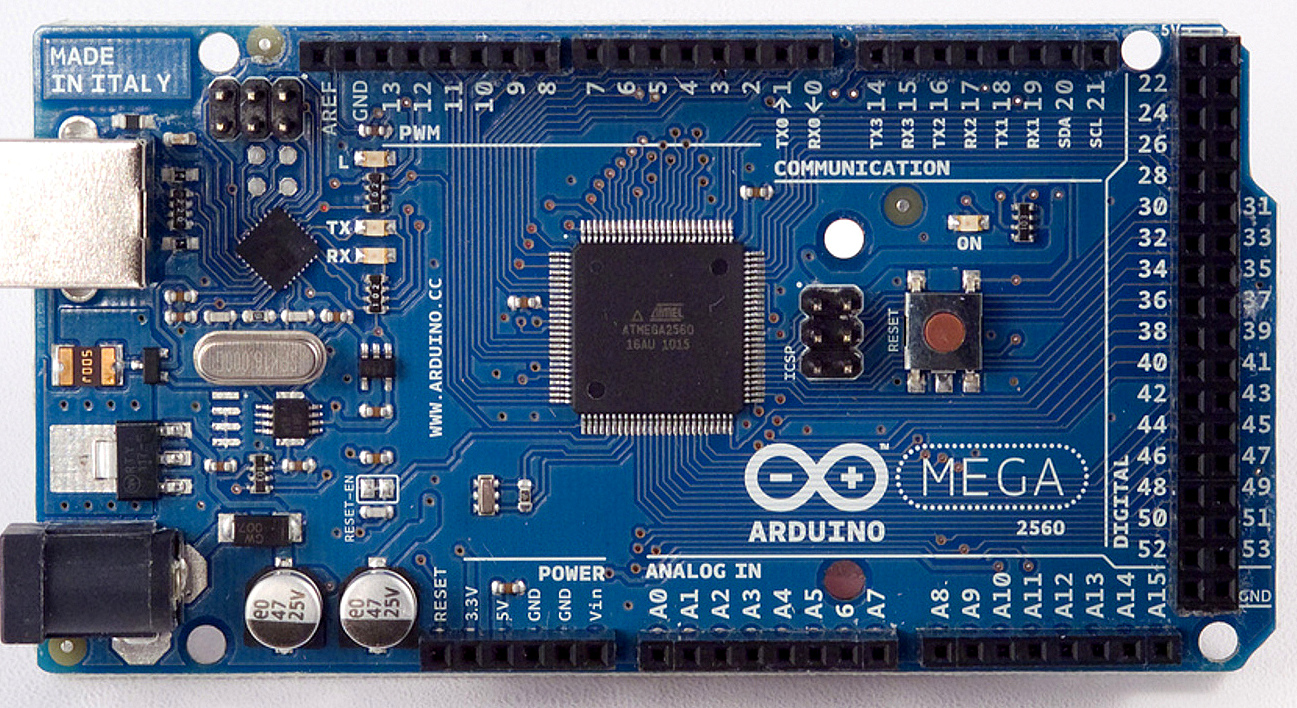
\includegraphics[width=0.9\textwidth]{img/arduino/arduinomega.jpg}
			\caption{Arduino Mega 2560.}
			\label{fig:arduinoHardware}
		\end{figure}
	\end{frame}
	\begin{frame}%{IDE Arduino 1.6.5}
		\begin{figure}[p]
			\centering
			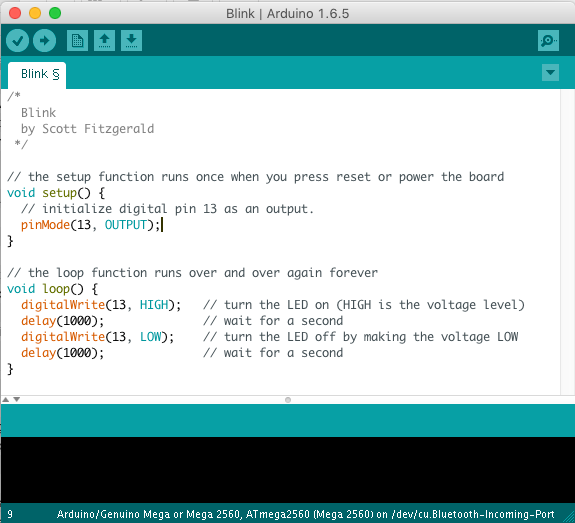
\includegraphics[width=0.72\textwidth]{img/arduino/ide.png}
			\caption{IDE Arduino 1.6.5.}
			\label{fig:arduinoHardware}
		\end{figure}
	\end{frame}
	\begin{frame}{Arduino}
		\begin{itemize}
			\item Características do Arduino utilizado no trabalho:
			\bigskip
			\begin{itemize}
  				\setlength\itemsep{0.9em}
				\item \textbf{Arduino Mega 2560} com microcontrolador ATmega2560;
				\item Possui 54 portas de entrada e saída Digital:
				\begin{itemize}
					\item Sendo 15 podendo ser utilizadas para saída PWM (\textit{Pulse-Width Modulation}).
				\end{itemize}
				\item Outras 16 portas para entrada analógica;
				\item Frequência de \textit{Clock} de $16 MHz$.
				%\item Memória?
			\end{itemize} 
		\end{itemize}
	\end{frame}


	\subsubsection{Linux}
	\begin{frame}{Linux}
		\centering \color{blue} {\Huge \textbf{Linux} \\[0.5cm]}% {\huge FPGA}
	\end{frame}
	% https://pt.wikipedia.org/wiki/Linux
	\begin{frame}{Linux}
		\begin{itemize}
			\setlength\itemsep{0.9em}
			\item \textbf{Linux} é um termo utilizado para referir sistemas operacionais que utilizam o \textbf{kernel Linux}.
			\item O sistema operacional como um todo tem como nome \textbf{GNU/Linux}. 
			\item Linux Kernel foi desenvolvido por Linus Torvalds em 1991.
			\item Reimplementação reelaborada do MINIX\footnote{Baseado no UNIX.} obedecendo o padrão POSIX \cite{nemeth2004manual}.
			\item Hoje é desenvolvido/estudado em projetos colaborativos de código-fonte aberto com principalmente:
			\begin{itemize}
				\setlength\itemsep{0.5em}
				\item Programadores individuais/Entusiastas;
				\item Colaborações de grandes empresas como \textit{IBM, Sun Microsystems, HP, Oracle, Google}, entre outras.
			\end{itemize}
		\end{itemize}
	\end{frame}
	\begin{frame}{Linux}
		\begin{itemize}
			\setlength\itemsep{1em}
			%\item Qualquer pessoa pode utilizar, estudar, modificar e distribuir o sistema segundo a licensa GPL\footnote{Executar e modificar desde que ajude ao seu próximo.}.
			\item Linux é um kernel \textbf{monolítico} no qual os \textit{Drivers} podem:
			\begin{itemize}
				\setlength\itemsep{0.7em}
				\item Executar com acesso total ao \textit{hardware};
				\item Configurados como módulos e carregados/descarregados \textbf{enquanto o sistema está ligado}.
			\end{itemize}
			\item Executa em arquiteturas como: \textit{Intel, StrongARM, PowerPC, Alpha}, etc. além de embarcados.
			\item Hoje, é possível encontrar distribuições Linux com coleções de \textit{software} (por exemplo o GNU) pronto para o uso \cite{campos}.
			%\item Uma das vantagens do sistema operacional livre é que seus módulos estão disponíveis para estudo.
			%\item Escrever um programa em espaço de usuário para torna-se mais fácil com uso de um \textit{Driver}.
		\end{itemize}
	\end{frame}
	\begin{frame}{Linux}
		\begin{multicols}{2}
				A distribuição Linux utilizada para a realização do desenvolvimento:
				\bigskip
				\begin{itemize}
					\item \textbf{Linux Mint 17.2} com codinome Rafaela, 64-bits;
				\end{itemize}
				\begin{figure}[p]
					\centering
					
\includegraphics[width=0.27\textwidth]{img/linux/mint.jpg}
					\caption{Logo Linux Mint.}
					\label{fig:mint}
				\end{figure}
			\columnbreak
				Sendo executado na máquina virtual:%
				\bigskip
				\begin{itemize}
					\item \textbf{Oracle VM VirtualBox 5.0.8} instalada no OS X El Capitan.
				\end{itemize}
				\begin{figure}[p]
					\centering
					
\includegraphics[width=0.25\textwidth]{img/linux/vm.png}
					\caption{Logo Oracle VM VirtualBox.}
					\label{fig:vb}
				\end{figure}
		\end{multicols}
	\end{frame}



	\subsection{Protocolos}
	\begin{frame}{Comunicação Serial}
		\begin{itemize}
			\setlength\itemsep{2.2em}
			\item Utilizadas a mais de 40 anos para a comunicação entre dispositivos \cite{nemeth2004manual}.
			\item São representadas por arquivos de dispositivo no diretório \texttt{ /dev}.
			%\begin{itemize}
			%	\item O nome dos arquivos é relevante somente para o usuário. O mapeamento é determinado pelos números Major e Minor.
			%\end{itemize}
			\item Foram utilizados dois protocolos de comunicação serial sendo eles:
			\begin{itemize}
				\setlength\itemsep{1em}
				\item UART;
				\item USB.
			\end{itemize}
		\end{itemize}
	\end{frame}
	\begin{frame}{Protocolos - UART}
		\begin{itemize}
			\item \textit{\textbf{U}niversal \textbf{A}synchronous \textbf{R}eceiver/\textbf{T}ransmitter}.
		\end{itemize}
		\bigskip
		\begin{figure}[p]
			\centering
			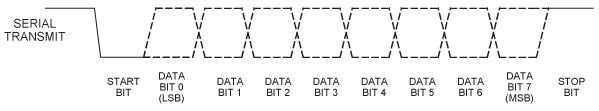
\includegraphics[width=1\textwidth]{img/fpga/uart.png}
			\caption{Protocolo de comunicação UART.}
			\label{fig:uart}
		\end{figure}
	\end{frame}
	\begin{frame}{Protocolos - USB}
	%\todo{Rever esse slide pra que fique mais fácil o entendimento}
		\begin{itemize}
			\setlength\itemsep{1em}
			\item \textbf{Atributos:} \textit{idVendor}, \textit{idProduct}, Números de \textit{Interfaces}, \textit{Endpoints}...
			\item \textbf{Um dispositivo USB possui:} \textit{Configurations}, \textit{Interfaces} e \textit{Endpoints}.
			\item Modo de envio de pacotes \textbf{por meio (ou não)} de \textbf{URB\footnote{\textit{\textbf{U}SB \textbf{R}equest \textbf{B}lock}.}}:
			\begin{itemize}
				\setlength\itemsep{0.7em}
				\item \textbf{Tipo:} Interrupt, Bulk, Control, Isochronous;
				\item \textbf{Operações:} Criar, destruir, enviar, callback handler, cancelamento.
			\end{itemize}
			\item Entre muitas outras características.
		\end{itemize}
	\end{frame}
	\begin{frame}
		\begin{figure}[p]
			\centering
			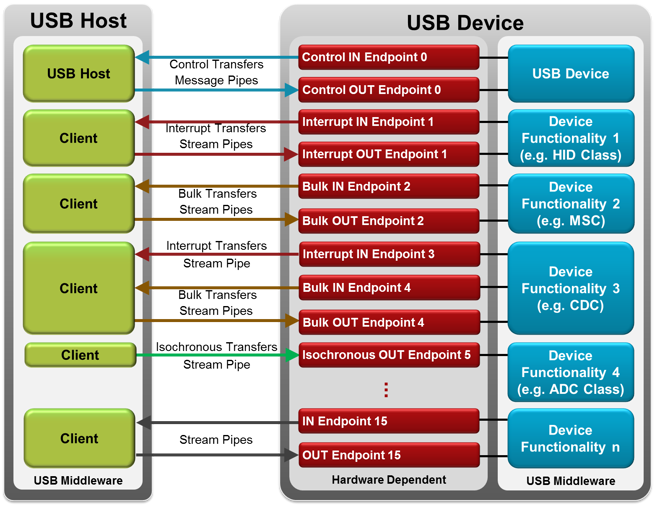
\includegraphics[width=0.87\textwidth]{img/endpoint2.png}
			\caption{Exemplo de comunicação USB.}
			\label{fig:uart}
		\end{figure}
	\end{frame}
	\begin{frame}{Protocolos - USB}
		\begin{itemize}
			\setlength\itemsep{1em}
			\item \textbf{Vantagens:}
			\begin{itemize}
				\setlength\itemsep{0.7em}
				\item \textit{Universal Serial Bus} é um sistema de \textbf{interconexão de periféricos genéricos}.
				\item \textbf{Cabos e conectores padronizados} além de vários \textbf{adaptadores} para extender suas funcionalidades.
				\item É um excelente sistema e que acredita-se durar ainda por vários anos \cite{nemeth2004manual}.
				\item O Linux tem um \textbf{amplo e sólido suporte} ao USB.
			\end{itemize}
			\item \textbf{Desvantagem:}
			\begin{itemize}
				\item Protocolo complexo.
			\end{itemize}
		\end{itemize}
	\end{frame}
	\begin{frame}{\textit{Driver} TTY}
		\begin{itemize}
			\item Abreviatura de \textit{\textbf{t}ele\textbf{t}\textbf{y}pewriter}.
			\item Interligava um terminal (físico ou virtual) a uma máquina Unix.
			\item Meio de nomear qualquer dispositivo de porta serial \cite{corbet2005linux}:
			\begin{itemize}
				\item \textbf{Físicos:}
				\begin{itemize}
					\item Portas Seriais;
					\item Conversores USB/serial;
					\item \textit{Modems} que necessitam de um processamento especial.
				\end{itemize}
				\item \textbf{Virtuais:}
				\begin{itemize}
					\item Consoles virtuais utilizados para fazer login em um computador por meio de uma conexão de rede;
					\item Entre outros.
				\end{itemize}
			\end{itemize}
			\item Vive \textbf{sob} o \textit{Driver} de Caractere e oferece \textbf{recursos de interface}:
			\begin{itemize}
				\item Controla o fluxo de dados;
				\item Formato dos dados.
			\end{itemize}
			\item Foco na \textbf{trasmissão e recebimento de dados com o \textit{hardware}}:
			\begin{itemize}
				\item Ao invés da interação com o espaço do usuário.
			\end{itemize}
		\end{itemize}
	\end{frame}
	\begin{frame}{\textit{Driver} TTY}
		%http://www.linusakesson.net/programming/tty/
		\begin{itemize}
			\item O \textbf{\textit{Driver} TTY}:
			\begin{itemize}
				\item Não comunica diretamente com o TTY \textit{Line Discipline};
				\item Formata os dados pro envio ao \textit{hardware} e também os recebe.
			\end{itemize}
			\item \textbf{TTY \textit{Line Discipline}}:
			\begin{itemize}
				\item Formatar os dados recebidos pelo usuário ou o \textit{hardware}, de forma específica (PPP, Bluetooth por exemplo).
			\end{itemize}
		\end{itemize}
		\begin{figure}[p]
			\centering
			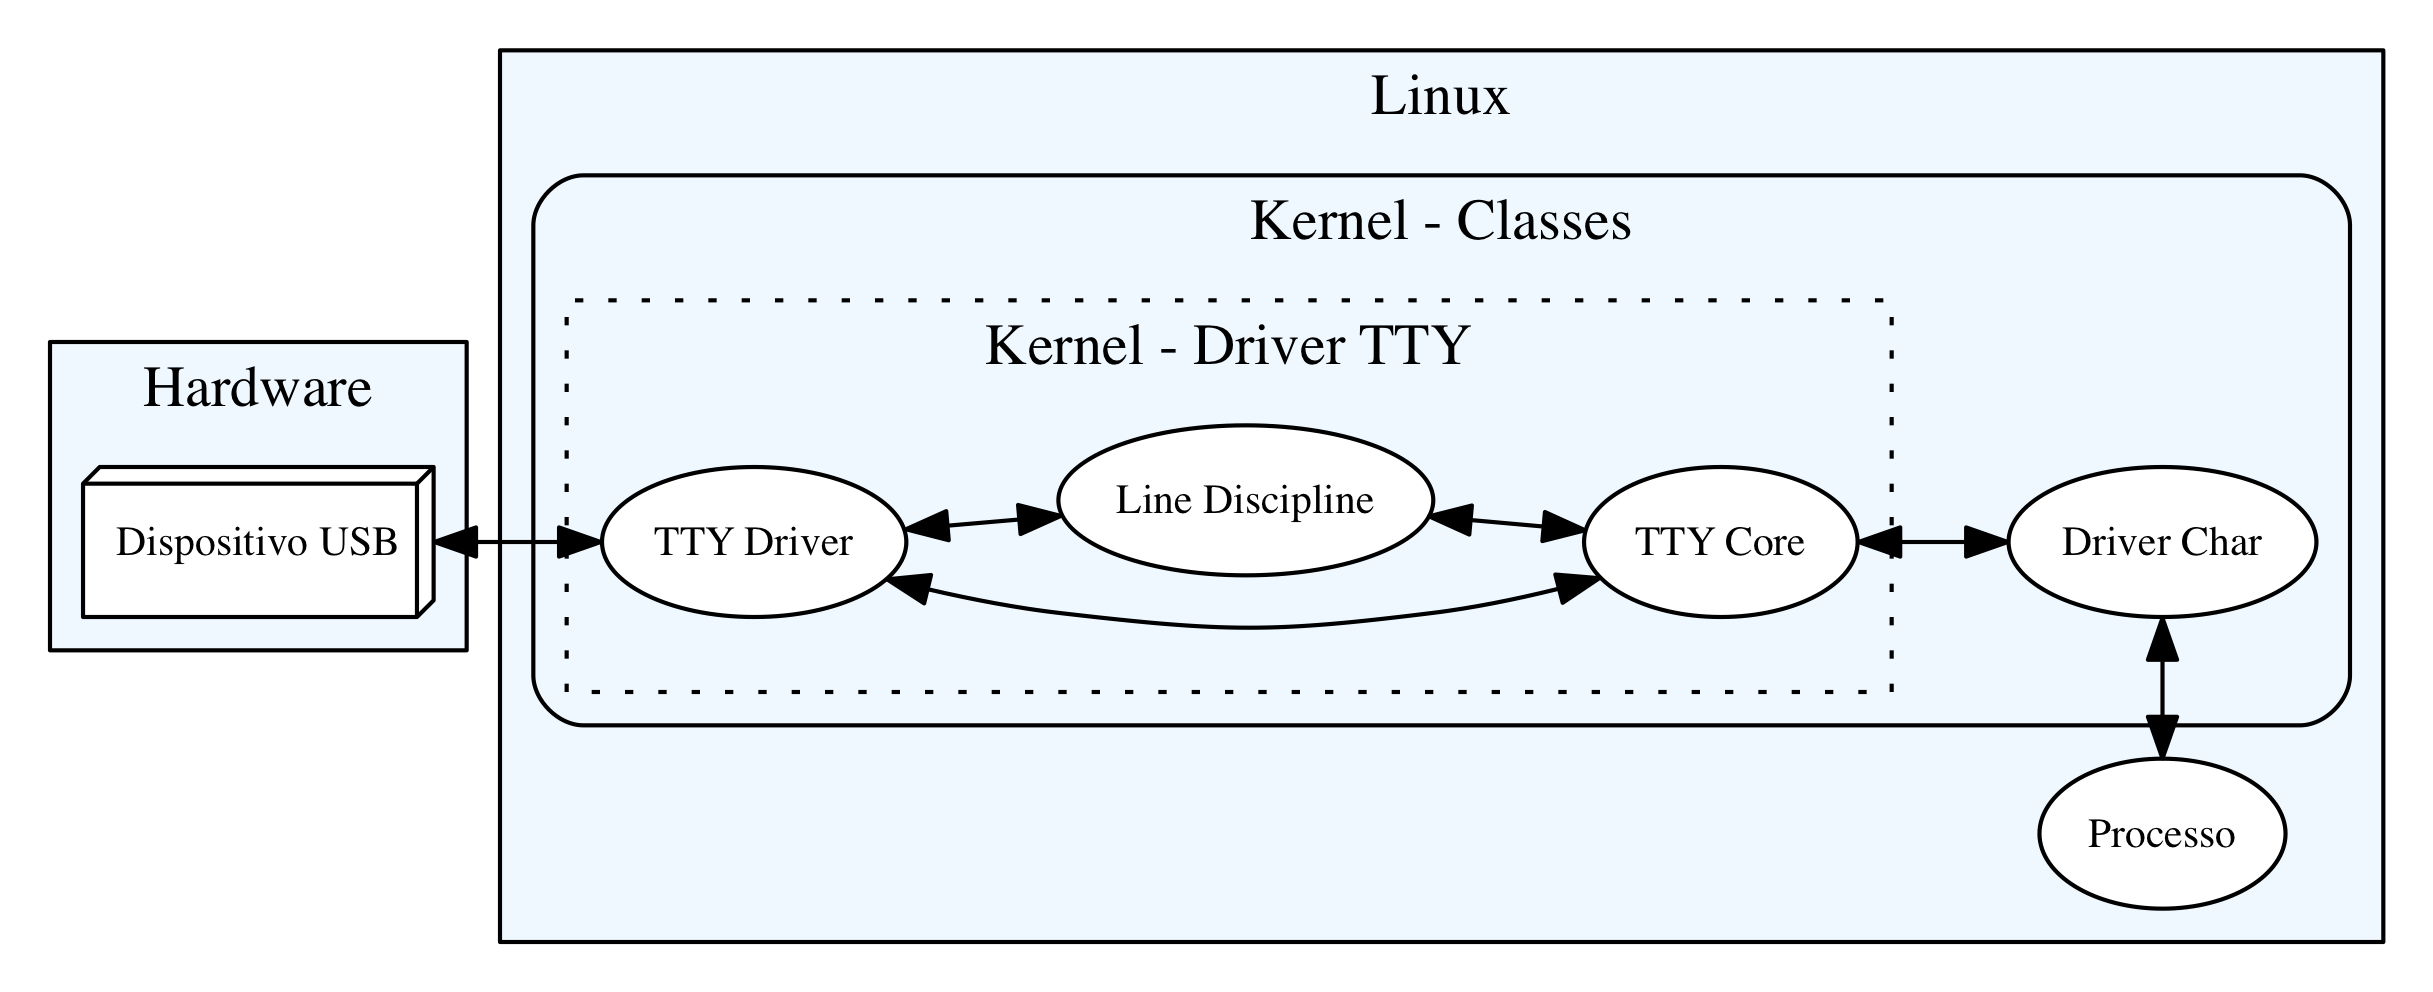
\includegraphics[width=0.85\textwidth]{img/tty.png}
			\caption{Comunicação utilizando TTY.}
			\label{fig:tty}
		\end{figure}
	\end{frame}

